\chapter{Ανάλυση Απαιτήσεων Συστήματος}

\section{Λειτουργικές Απαιτήσεις}
\subsubsection{Έξοδοι του Συστήματος}
Στο σύστημα, αποδέκτες των εξόδων αποτελούν όλοι οι χρήστες του, δηλαδή οι πελάτες, οι καμαριέρες 
και καθώς και ο υπάλληλος υποδοχής. Παρακάτω αναγράφονται επιγραμματικά τα στοιχεία εξόδου 
ανάλογα με τον αποδέκτη του. 

\noindent \\ 
Στον πελάτη παρέχονται οι παρακάτω έξοδοι:
\begin{itemize}
	\item  Λίστα με προσφερόμενα γεύματα.
	\item  Λίστα πληροφοριών για την πόλη των Χανίων.
	\item  Προβολή ερωτήσεων που δέχεται από τον υπεύθυνο υποδοχής.
	\item  Προβολή απαντήσεων  που δέχεται από τον υπεύθυνο υποδοχής.		
	\item  Pop-up window κατά την αναμονή έγκρισης/απόρριψης της παραγγελίας.
\end{itemize}

\noindent \\
Στον υπάλληλο υποδοχής παρέχονται οι παρακάτω έξοδοι:
\begin{itemize}
	\item  Pop-up window σχετικά με την επεξεργασία των FAQ
	\item Προβολή ερωτήσεων που δέχεται από τον υπεύθυνο υποδοχής.
	\item Προβολή απαντήσεων  που δέχεται από τον υπεύθυνο υποδοχής.	
\end{itemize}

\noindent \\ 
Στις καμαριέρες παρέχονται οι παρακάτω έξοδοι:
\begin{itemize}
	\item  Pop-up window σχετικά με το αίτημα γεύματος από πελάτη.
	\item  Pop-up window σχετικά με την ολοκλήρωση  επαρκούς αριθμού δωματίων που καθαρίστηκαν.
\end{itemize}

\noindent \\ 
Ως αυτοματοποιημένη έξοδος, παρέχεται η εξής:
\begin{itemize}
	\item  Ανανέωση λίστας αντικειμένων προς ανανέωση
\end{itemize}

\begin{table}[H]
	\begin{tabular}{|c|c|c|c|c|}
		\hline
		\textbf{Έξοδος}       & \begin{tabular}[c]{@{}c@{}}Pop-up window \\ κάθε είδους\end{tabular} & Λίστες Πληροφοριών & Ερωτήσεις  & Απαντήσεις   \\ \hline
		\textbf{Τύπος Εξόδου} & Γραφική Διεπαφή                                                      & Γραφική Διεπαφή    & Απλό κείμενο & Απλό κείμενο \\ \hline
	\end{tabular}
\end{table}
\clearpage

\noindent\\
Αναφορικά με τον λόγο που παράγεται κάθε έξοδος, η προβολή ερωτήσεων και απαντήσεων
μεταξύ δύο χρηστών παράγεται μετά την έναρξη προσωπικής συνομιλίας από έναν χρήστη. Τα pop-up
Windows, παράγονται από τον πελάτη κατά την παραγγελία φαγητού ώστε να τον ενημερώσουν για
την έγκριση ή την απόρριψη της παραγγελίας του, στην καμαριέρα ώστε να εγκρίνει ή να  απορρίψει 
μία παραγγελία αλλά και στις περιπτώσεις όπου συμπλήρωσε τον απαιτούμενο αριθμό δωματίων τα 
οποία καθάρισε και στον υπάλληλο υποδοχής εφόσον επιτυχώς ενημέρωσε την λίστα με τις 
συχνές ερωτήσεις. Ακόμα, οι λίστες παράγονται σε περίπτωση που ο πελάτης θελήσεις να πληροφορηθεί 
σχετικά με τα Χανιά  ή στην περίπτωση που αιτηθεί παραγγελία γεύματος όπου και εμφανίζεται μία λίστα
με τα προσφερόμενα γεύματα. Τέλος, η αυτοματοποιημένη έξοδος που αναγράφεται, αναφέρεται στην 
αυτοματοποιημένη λειτουργία κατά την οποία το πρόγραμμα προσθέτει αντικείμενα στην λίστα 
παραγγελιών  του καταλύματος εαν βρεθεί πως υπάρχει έλλειψη μετά από έλεγχο των δεδομένων που 
εισήγαγε η καμαριέρα κατά τον καθαρισμό του δωματίου.\\

\noindent
Όσον αφορά τη γραφική διεπαφή pop-up window, είναι ένα παράθυρο τύπου pop-up στο οποίο εμφανίζεται
ένα μήνυμα σχετικό με το λόγο που παράχθηκε σε κάθε περίπτωση καθώς και ένα ή δύο κουμπιά για την 
υλοποίηση επιμέρους διαδικασιών. Ενδεικτικά, στην περίπτωση έγκρισης παραγγελίας, αναγράφονται τα 
ζητούμενα γεύματα και υπάρχουν δύο κουμπιά με τα οποία μπορεί να εγκρίνει ή να απορρίψει της. 


\subsubsection{Είσοδοι του Συστήματος}
Οι είσοδοι του συστήματος χωρίζονται ανάλογα με το είδος του χρήστη. Λόγω της φύσης του 
συστήματος, οι χρήστες του συστήματος είναι οι πελάτες του καταλύματος, ο υπεύθυνος υποδοχής 
καθώς και οι καμαριέρες και ο κάθε ένας έχει τη δυνατότητα εκτέλεσης διαφορετικών διαδικασιών και ως
αποτέλεσμα, εισαγωγή διαφορετικών εισόδων σε αυτό.  Λόγω της φύσης του συστήματος, όλες οι 
είσοδοι προσλαμβάνονται από το σύστημα μέσω της οθόνης αφής κάθε συσκευής και στις περιπτώσεις
όπου απαιτείται η εισαγωγή κειμένου ή αριθμών, μέσω του πληκτρολογίου που εμφανίζεται σε αυτή.

\noindent \\ 
Στον πελάτη παρέχονται οι παρακάτω είσοδοι:
\begin{itemize}
	\item Σύνταξη μηνύματος ως ερώτηση σε προσωπική συνομιλία
	\item Σύνταξη μηνύματος ως απάντηση σε προσωπική συνομιλία
	\item Επιλογή γεύματος καθώς και αντίστοιχων πληροφοριών που ζητούνται κατά την παραγγελία
\end{itemize}

\noindent \\ 
Στον υπάλληλο υποδοχής παρέχονται οι παρακάτω είσοδοι:
\begin{itemize}
	\item Αλλαγή περιεχομένου FAQ
	\item Σύνταξη μηνύματος ως ερώτηση σε προσωπική συνομιλία
	\item Σύνταξη μηνύματος ως απάντηση σε προσωπική συνομιλία 
\end{itemize}

\noindent \\ 
Στην καμαριέρα παρέχονται οι παρακάτω είσοδοι:
\begin{itemize}
	\item Απόρριψη ή έγκριση παραγγελίας πελάτη
	\item Συμπλήρωση πλήθους αντικειμένου κάθε δωματίου
\end{itemize}


\subsubsection{Προτεραιότητες και Διαδικασίες του Συστήματος}
Το σύστημα έχει 6 προβλεπόμενες διαδικασίες οι οποίες φαίνονται στο παρακάτω High level use case διάγραμμα \ref{high_level_use_case}  
\begin{figure}[H]
	\centering
	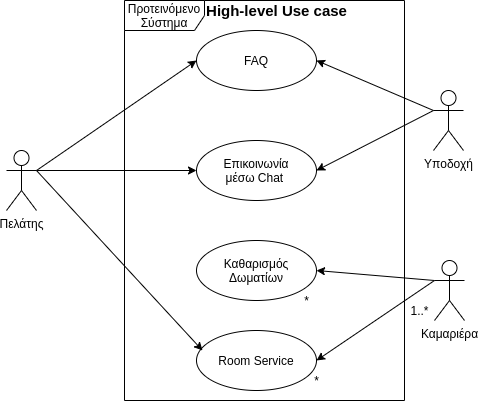
\includegraphics[width=0.5\textwidth]{Images/High_level_use_case}
	\caption{High Level Use Case Diagram}
	\label{high_level_use_case}
\end{figure}

\noindent
Οι επιμέρους διαδικασίες περιγράφονται παρακάτω συνοδευόμενες από τα Detailed use case κάθε μίας. \\

\noindent
Όσον αφορά την λειτουργία "Συχνών Ερωτήσεων" (FAQ) προβλέπονται δύο διαδικασίες που μπορούν να 
εκπονηθούν. Εμπλεκόμενοι σε αυτή τη λειτουργία είναι ο πελάτης και ο υπάλληλο υποδοχής. Όσον αφορά 
τον πελάτη αρχικά, γίνεται η επιλογή της λειτουργίας "FAQ" στο κεντρικό μενού και στη συνέχεια 
εμφανίζεται στον χρήστη μία λίστα με ερωτήσεις μαζί με τις απαντήσεις τους, από τις οποίες μπορεί να 
αντλήσει χρήσιμες πληροφορίες. Όσον αφορά τον υπάλληλο υποδοχής, αρχικά, γίνεται η επιλογή της 
λειτουργίας "Επεξεργασίας FAQ" στο κεντρικό μενού και στη συνέχεια δίνεται η δυνατότητα Προσθήκης
/Επεξεργασίας/Διαγραφής μίας ερώτησης ή της αντίστοιχης απάντησης της από την λίστα. Με την 
ολοκλήρωση  της επεξεργασίας, εμφανίζεται το αντίστοιχο  pop-up window.\\
\begin{figure}[H]
	\centering
	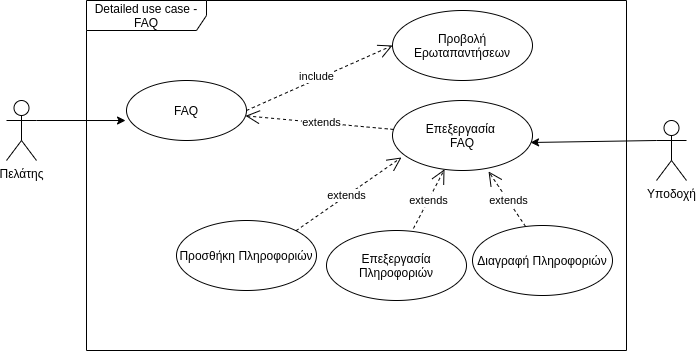
\includegraphics[width=0.7\textwidth]{Images/Low_level_use_case-FAQ}
	\caption{Low Level Use Case Diagram - FAQ}
	\label{Low_level_use_case - FAQ}
\end{figure}
\clearpage

\noindent
Όσον αφορά την λειτουργία "Room service".  Αρχικά,  γίνεται και πάλι επιλογή της από το κεντρικό
μενού και στην συνέχεια από τον χρήστη ζητείται η επιλογή του είδους γεύματος που επιθυμεί (Βραδινό ή 
Πρωινό). Μέσω αυτή της επιλογής, εμφανίζεται ο αντίστοιχος κατάλογος για το κάθε είδος όπου ο χρήστης 
κάνει την/τις  επιλογή/ες του. Τέλος,  ζητείται η ώρα παράδοσης αυτού και εφόσον έχει ολοκληρώσει την 
παραγγελία του, το αίτημα του αποστέλλεται ενώ εμφανίζεται το αντίστοιχο μήνυμα εξόδου ώστε ο χρήστης 
να γνωρίζει εάν το αίτημά του εγκρίθηκε ή απορρίφθηκε.  Αυτή η απάντηση δίνεται μία καμαριέρα που βρίσκεται
σε βάρδια εκείνη την ώρα, η οποία ελέγχει εάν οι προμήθειες επαρκούν και ανάλογα με αυτές, εγκρίνει ή 
απορρίπτει το αίτημα του πελάτη. Αυτό, γίνεται μέσω της ειδοποίησης που εμφανίστηκε σε αυτή.  Σε περίπτωση
απόρριψης, ο πελάτης έχει την δυνατότητα δημιουργίας νέας παραγγελίας εάν το επιθυμεί.\\
\begin{figure}[H]
	\centering
	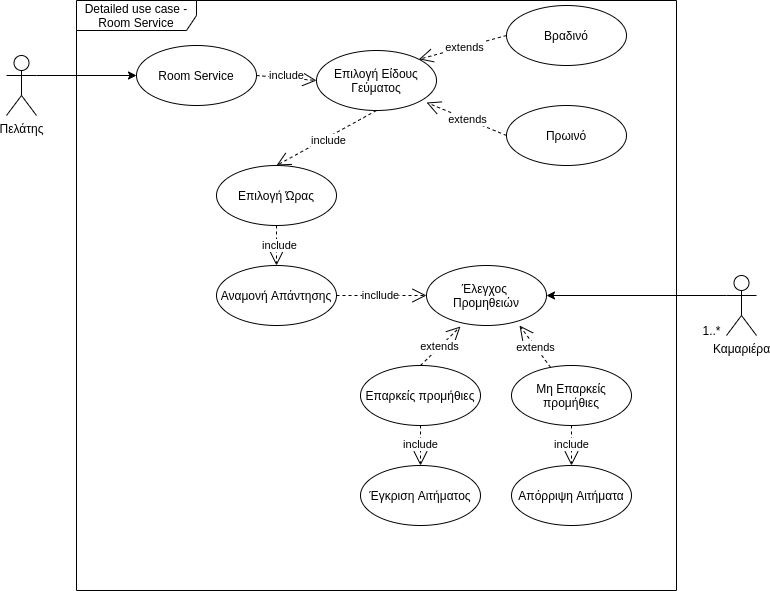
\includegraphics[width=0.7\textwidth]{Images/Low_level_use_case-Room service}
	\caption{Low Level Use Case Diagram - Room Service}
	\label{Low_level_use_case - Room Service}
\end{figure}
\clearpage

\noindent
H Τρίτη διαδικασία είναι η "Επικοινωνία με την Reception".  Αρχικά, γίνεται και πάλι η επιλογή της στο κεντρικό 
μενού και στη συνέχεια το γραφικό περιβάλλον αλλάζει και γίνεται σαν ένα κοινό chat room.  Μέσω αυτού, 
έχει την δυνατότητα να πληκτρολογεί μηνύματα και να δέχεται απαντήσεις από τον υπεύθυνο υποδοχής σε 
πραγματικό χρόνο. Κατά την αποστολή ενός μηνύματος, από τον πελάτης προς τον χρήστη, ο υπεύθυνος 
υποδοχής  δέχεται μία ειδοποίηση μηνύματος μέσω της οποίας μπορεί να μεταβεί και αυτός στο ίδιο γραφικό
περιβάλλον και να συνομιλήσει με τον πελάτη.  \\

\noindent
Η τέταρτη διαδικασία είναι η "Αναφορά Δωματίων".  Αρχικά, γίνεται η επιλογή της στο κεντρικό  μενού και 
στη συνέχεια ζητείται η προσθήκη του αριθμού δωματίου στο οποίο έγιναν οι απαραίτητοι έλεγχοι καθώς και 
τα προβλεπόμενα πρωτόκολλα καθαρισμού. Στη συνέχεια, εμφανίζεται μία λίστα με όλα τα αντικείμενα τα οποία
αναμένεται να υπάρχουν στο δωμάτιο. Στη λίστα αυτή δίνεται η δυνατότητα για κάθε ένα από τα αντικείμενα, να 
συμπληρωθεί  ο αριθμός που βρέθηκε στο δωμάτιο. Σε περίπτωση που κάποιο αντικείμενο απουσιάζει, δηλαδή 
δηλώνεται μικρότερος αριθμός από τον αναμενόμενο, αυτό προστίθεται μέσω έτοιμου κώδικα σε ένα αρχείο τύπου
csv, ώστε να μπορεί να γίνει η αντίστοιχη παραγγελία στους προμηθευτές. Αυτή η διαδικασία επαναλαμβάνεται 
έως ότου η καμαριέρα συμπληρώσει τον προβλεπόμενο αριθμό δωματίων που έχει αναλάβει.\\

\noindent 
Η πέμπτη και τελευταία διαδικασία είναι η "Επικοινωνία με τον Πελάτη". Η παρούσα διαδικασία παρουσιάζει πολλές 
ομοιότητες  με την αντίστοιχη λειτουργία  για πελάτες, με μόνη διαφορά πως στον υπεύθυνο υποδοχή, κατά την επιλογή 
της διαδικασίας , εμφανίζεται μία λίστα με όλα τα δωμάτια του ξενοδοχείου και μέσω αυτής επιλέγει με ποιό απ'όλα 
επιθυμεί να συνομιλήσει.\\

\noindent
Τέλος, όσον αφορά τις προτεραιότητες, από την περιγραφή των διαδικασιών είναι εμφανές πως  μόνο στην δεύτερη
στην τρίτη και στην τέταρτη διαδικασία για να εμπλακεί και ο δεύτερος χρήστης είναι απαραίτητο να έχουν γίνει 
κάποια απαραίτητα βήματα. Πιο συγκεκριμένα στην δεύτερη διαδικασία, για να εμπλακεί και η καμαριέρα, είναι 
απαραίτητο ο πελάτης να στείλει την παραγγελία του, ενώ στην τρίτη και την τέταρτη, για να εμπλακεί ο δεύτερος 
χρήστης είναι απαραίτητο ο πρώτος να αιτηθεί συνομιλία μαζί του.

\section{Μή Λειτουργικές Απαιτήσεις}
